\documentclass[11pt]{article}
\usepackage[utf8]{inputenc}
\usepackage{graphicx}
\usepackage{titling}
\usepackage{index}
\usepackage{fancyhdr}
\usepackage{enumitem}
\usepackage{microtype}
\usepackage{blindtext}
\usepackage{amsmath}
\usepackage{wrapfig}
\usepackage[labelformat=empty]{caption}
\usepackage{listings}
\usepackage{xcolor}

\definecolor{codegreen}{rgb}{0,0.6,0}
\definecolor{codegray}{rgb}{0.5,0.5,0.5}
\definecolor{codepurple}{rgb}{0.58,0,0.82}
\definecolor{backcolour}{rgb}{0.95,0.95,0.92}

\lstdefinestyle{mystyle}{
    backgroundcolor=\color{backcolour},   
    commentstyle=\color{codegreen},
    keywordstyle=\color{magenta},
    numberstyle=\tiny\color{codegray},
    stringstyle=\color{codepurple},
    basicstyle=\ttfamily\footnotesize,
    breakatwhitespace=false,         
    breaklines=true,                 
    captionpos=b,                    
    keepspaces=true,                 
    numbers=left,                    
    numbersep=5pt,                  
    showspaces=false,                
    showstringspaces=false,
    showtabs=false,                  
    tabsize=2
}

\lstset{style=mystyle}

\pretitle{
\begin{center}
\vspace{2.5cm}


\includegraphics[scale=0.2]{FEUP_LOGO.png}

\vspace{2cm}

\LARGE \textbf{Redes de Computadores}

\vspace{0.5cm}

}
\posttitle{\end{center}}

\title{\large{\textbf{Ligação de Dados}} }
\author{Nuno Miguel Fernandes Marques - 201708997 - MIEIC}
\date{\today}

\begin{document}
\maketitle
\thispagestyle{empty}

\newpage
\thispagestyle{fancy}
\fancyhf{}
\fancyhead[R]{Ligação de dados}
\fancyfoot[R]{\thepage}
\renewcommand*{\footrulewidth}{1pt}

\section*{Sumário}
Este relatório e feito no âmbito do primeiro trabalho laboratorial de Redes de computadores. O trabalho consiste na transmissão de ficheiros usando a porta de série. As principais conclusões obtidas neste projeto foram:
\begin{itemize}
    \item As relações de tamanho da trama e erro em tramas com a eficiência da ligação.
    \item A eficiência da transmissão de dados pela porta de séria, até \empth{79\%} neste projeto.
    \item A necessidade de camadas independentes na transmissão de dados em redes de computadores.
\end{itemize}
  

\section*{Introdução}
Este projeto tinha como objectivo final desenvolver e testar uma aplicação com objectivo de realizar a \textbf{transmissão de ficheiros pela porta de série} fazendo o uso de duas camadas independentes, a ligação de dados e a aplicação.
Este relatório está divido nas seguintes secções:
\begin{itemize}
    \item \textbf{Arquitetura} - Blocos funcionais e interfaces
    \item \textbf{Estrutura do código} - API, estruturas de dados e funções
    \item \textbf{Casos de uso principais} - Casos de uso do projeto e sequências de chamada de funções
    \item \textbf{Protocolo de ligação lógica} - Descrição dos aspetos funcionais e estratégias usadas na camada da ligação
    \item \textbf{Protocolo de aplicação}- Descrição dos aspetos funcionais e estratégias usadas na camada da aplicação
    \item \textbf{Validação} - Validações efectuadas
    \item \textbf{Eficiência do protocolo de ligação de dados} - Medição e análise da eficiência do protocolo usado
    \item \textbf{Conclusões} - Resumo das conclusões sobre o projeto e sobre o tema apresentado.
\end{itemize}


\newpage
\thispagestyle{fancy}
\fancyhf{}
\fancyhead[R]{Ligação de dados}
\fancyfoot[R]{\thepage}
\renewcommand*{\footrulewidth}{1pt}

\section*{Arquitetura}
Existem dois \textbf{blocos funcionais} independentes no trabalho, o bloco da \textbf{ligação de dados} e o bloco da \textbf{aplicação}. O bloco de ligação de dados tem como objectivo abrir e fechar a ligação, assegurar a transmissão correta das tramas e recuperação quando ocorrem erros de transmissão. Este bloco tem um nível baixo fazendo a ligação diretamente com a porta de série.
\newline
\newline
O Bloco da aplicação tem como objectivo ler e escrever ficheiros, gerir o tamanho das tramas de dados e assegurar que os dados recebidos são válidos. Este bloco tem um nível mais alto fazendo uso da API definida no bloco da ligação de dados.\\\\
Ambos os blocos fazem uso de um \textbf{\empth{array dinâmico}} na sua gestão de memória.
\newline
\newline
A \textbf{interface} permite o uso do mesmo executável para recepção e transmissão, especificando a opção na linha de comandos. Alem disso e necessário especificar o nome do ficheiro a transmitir e a porta de série a usar. \underline{Baudrate}, tamanho máximo das tramas, número máximo de tentativas de retransmissão e tempo limite sem comunicação são definições opcionais. O progresso da transmissão e mostrada usando uma barra de progresso. No fim são apresentadas as estatísticas da transmissão.\\\\
\begin{figure}[!ht]
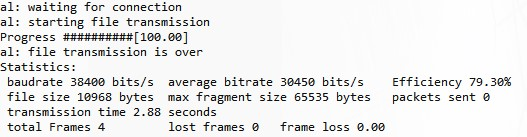
\includegraphics[scale=1]{INTERFACE.jpg}
\caption{\scriptsize Exemplo do output de uma execução}
\end{figure}

\newpage
\thispagestyle{fancy}
\fancyhf{}
\fancyhead[R]{Ligação de dados}
\fancyfoot[R]{\thepage}
\renewcommand*{\footrulewidth}{1pt}

\section*{Estrutura do código}
\textbf{Camada de ligação}\\
A \emph{API} da camada de ligação disponibiliza as seguintes funções:\\
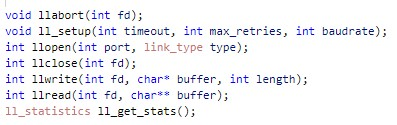
\includegraphics[scale=1]{LLAPI.jpg}\\
E internamente usa as seguintes estruturas de dados:\\
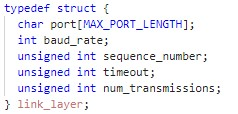
\includegraphics[scale=1]{LLSTRUCT.jpg}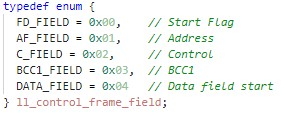
\includegraphics[scale=1]{LLCFF.jpg}\\
\textbf{Camada da Aplicação}\\
A camada de ligação disponibiliza as seguintes funções:\\
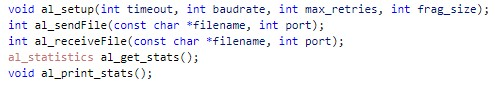
\includegraphics[scale=1]{ALFUN.jpg}\\
E internamente usa as seguintes estruturas de dados:\\
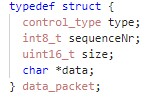
\includegraphics[scale=1]{ALDATA.jpg}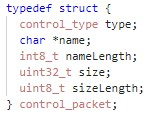
\includegraphics[scale=1]{ALCONTROL.jpg}\\

\newpage
\thispagestyle{fancy}
\fancyhf{}
\fancyhead[R]{Ligação de dados}
\fancyfoot[R]{\thepage}
\renewcommand*{\footrulewidth}{1pt}

\section*{Casos de uso principais}
A \textbf{camada de ligação} terá como casos de uso principais permitir uma aplicação \textbf{ligar} a porta de série\textbf{\empth{(llopen)}}, \textbf{enviar ou receber} segmentos de dados\textbf{\empth{(llread e llwrite)}} e \textbf{desligar a ligação}\textbf{\empth{(llclose)}}. Alem disso disponibiliza estatísticas sobre a ligação, neste caso tramas totais enviadas e tramas perdidas. Esta camada pode ser configurada com uso da função \textbf{\emph{ll\_setup}}, sendo possível alterar o \emph{baudrate}, o número máximo de retransmissões e o tempo limite para retransmissão.
\\\\
A camada da aplicação tem dois casos de uso principais: \textbf{enviar ou receber} um ficheiro usando as funções \textbf{\empth{al\_sendFile}} e \textbf{\empth{al\_receiveFile}} respectivamente. Esta camada pode ser configurada com o uso da função \textbf{\empth{al\_setup}} que permite configurar o tamanho máximo de cada segmento de dados individual. Esta camada disponibiliza também estatísticas sobre \empth{bits} por segundo médio, quantidade de segmentos de dados enviados, duração da transmissão e eficiência em relação ao valor máximo teórico de transmissão.
\\\\
No caso de receção a função \textbf{\empth{al\_receiveFile}} faz uso das funções: \textbf{\empth{llopen}}, \textbf{\empth{llread}} e \textbf{\empth{llclose}} da camada de ligação.\\
No caso de emissão a função \textbf{\empth{al\_sendFile}} faz uso das funções \textbf{\empth{llopen}}, \textbf{\empth{llwrite}} e \textbf{\empth{llclose}} da camada de ligação


\section*{Protocolo de ligação lógica}
O protocolo de ligação de dados começa pela função \textbf{\empth{llopen}}, esta função começa por abrir a ligação com a porta de série usando as configuração fornecidas. Após estabelecer a ligação, o receptor espera que o emissor envie uma trama de controlo \empth{SET}, ao enviar a trama de controlo \empth{SET}, o emissor fica a espera de uma trama de controlo \empth{UA} como resposta.\\

Após essa comunicação é possível começar a transmissão de tramas de dados usando \textbf{\empth{(llread e llwrite)}}. Em \textbf{\empth{llwrite}} o cabeçalho da trama de dados é criado, depois o segmento de dados é introduzido na trama \empth{byte} a \empth{byte}. Simultâneamente e calculado o byte de segurança \textbf{BCC2} e é feito o \textbf{\empth{byte stuffing}}, finalmente é verificado se o \textbf{BCC2} precisa \textbf{\empth{byte stuffing}} e é introduzido na trama. Com a trama completa é feito o envio pela porta de séria, uma trama de controlo \empth{RR} é esperada em resposta. Caso a resposta demore mais que o tempo limite, a trama \empth{RR} seja duplicada ou seja uma
\newpage
\thispagestyle{fancy}
\fancyhf{}
\fancyhead[R]{Ligação de dados}
\fancyfoot[R]{\thepage}
\renewcommand*{\footrulewidth}{1pt}
resposta do tipo \empth{REJ} a retransmissão da trama é feita. No caso de ultrapassar o limite de retransmissões a operação é abortada.\\~
\begin{figure}[h!]
  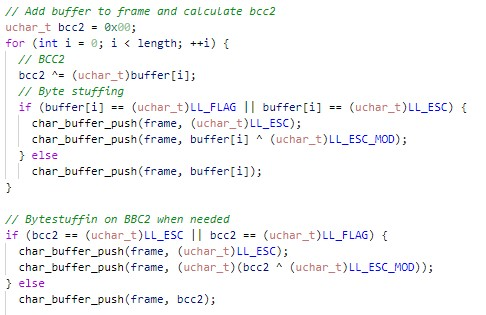
\includegraphics[scale=0.8]{BYTESTUFFING.jpg}
  \caption{Calculo de BCC2 e byte stuffing}
\end{figure}
\\
Em \textbf{\empth{llread}} é esperada uma trama de dados. Ao receber a trama o cabeçalho é validado, e os dados são lidos \empth{byte} a \empth{byte}, fazendo o \textbf{\empth{byte destuffing}} quando necessário e calculando o \textbf{BCC2} esperado ao mesmo tempo. Depois deste processo o \textbf{BCC2} é lido e comparado com o \textbf{BCC2} esperado. Se este processo for feito sem problemas uma trama de controlo \empth{RR} é enviada. Caso seja encontrado um problema em qualquer dos passos uma trama de controlo \empth{REJ} é enviada.\\

Finalmente em \textbf{\empth{llclose}} o emissor envia uma trama de controlo \empth{DISC}, á qual o receptor responde também com \empth{DISC}. Neste ponto o emissor envia a trama de controlo \empth{UA} e encerra a ligação e repõe a configuração da porta de série. O receptor faz o mesmo após receber a trama de controlo \empth{UA}.

\newpage
\thispagestyle{fancy}
\fancyhf{}
\fancyhead[R]{Ligação de dados}
\fancyfoot[R]{\thepage}
\renewcommand*{\footrulewidth}{1pt}

\section*{Protocolo de aplicação}
O protocolo de aplicação tem um nível mais alto e faz uso da \empth{API} do protocolo de ligação de dados para efectuar transferências de ficheiros. Esta camada pode ser representa por apenas duas funçoes: \textbf{al\_receiveFile e al\_sendFile}. Ambas as funções inicialização e fecham a ligação no fim da operação.\\\\ A função \textbf{\empth{al\_sendFile}} lê o ficheiro e primeiro envia um pacote de controlo para sinalizar o inicio da transferência. Depois para cada segmento de dados é criado um pacote de dados que inclui o nome do ficheiro, número de sequência do pacote, tamanho do segmento e o próprio segmento, usando a função \empth{llwrite} da camada de ligação. Quando todos segmentos forem enviados, outro pacote de controlo é enviado para sinalizar o fim da transferência.\\\\

A função \textbf{\empth{al\_receiveFile}} usa a função \empth{llread} para ler estes pacotes. Á medida que recebe pacotes a função guarda os segmentos num ficheiro até receber o pacote de controlo a sinalizar o fim da transmissão. Esta função valida os números de sequência dos pacotes e, no fim, se recebeu a quantidade correta de \empth{bytes}.\\\\
Esta camada também calcula e disponibiliza \textbf{estáticas} da transmissão.


\section*{Validação}
Os seguintes testes foram aplicados neste trabalho:
\begin{itemize}
    \item Envio de ficheiros de tamanhos diferentes
    \item Interrupção de ligação em momentos aleatórios durante a transmissão
    \item Introdução de \empth{bits} aleatórios durante a transmissão
    \item Simulação de erros no \empth{BCC2} das tramas de dados
    \item Variação do \empth{baudrate}, número máximo de retransmissões, tempo até retransmissão e tamanho da trama
\end{itemize}
Pelo fim do projeto os testes foram realizados com sucesso.

\newpage
\thispagestyle{fancy}
\fancyhf{}
\fancyhead[R]{Ligação de dados}
\fancyfoot[R]{\thepage}
\renewcommand*{\footrulewidth}{1pt}

\section*{Eficiência do protocolo de ligação de dados}
Neste testes a efeciencia foi medida usando a formula \emph{S=(R/C)}.\\\\
\textbf{Variável: Capacidade de ligação (C) }\\
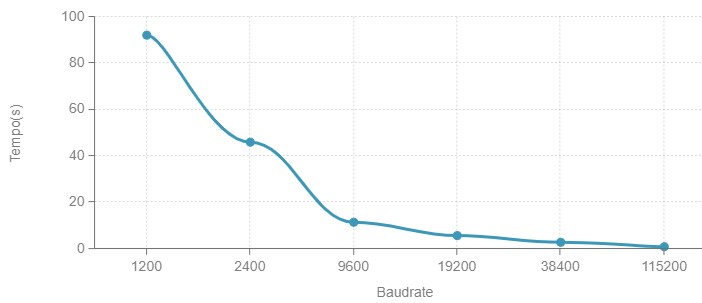
\includegraphics[scale=0.6]{CVAR.jpg}\\
Testes realizados com ficheiro de tamanho constante 10.7KB, com trama constante de 10KB. A \textbf{eficiência} manteve estável em todos testes, sendo sempre aproximadamente \textbf{79\%}.\\\\

\textbf{Variável: Tamanho da trama de dados}
\begin{center}
\scalebox{0.8}{
 \begin{tabular}{| c | c | c | c |} 
 \hline
 Tamanho(bytes) & Tempo(s) & R(bits/s) & S(R/C)(\%) \\ [0.5ex] 
 \hline\hline
 10 & 8.60 & 10199 & 23.56 \\ 
 \hline
 40 & 4.31 & 20359 & 53.02 \\
 \hline
 100 & 3.44 & 25486 & 66.37 \\
 \hline
 500 & 2.99 & 29348 & 76.43 \\
 \hline
 1000 & 2.93 & 29917 & 77.91 \\
 \hline
 4000 & 2.89 & 30340 & 79.01 \\ [1ex] 
 \hline
 10000 & 2.88 & 30416 & 79.21 \\ [1ex] 
 \hline
\end{tabular}}
\end{center}
Nestes testes foi usado um \emph{baudrate} constante de 38400 e uma imagem de tamanho constante 10.7KB. Nestes testes observamos que existe um ganho grande de eficiência a aumentar o tamanho da trama, para tamanhos pequenos. Mas a partir dos \textbf{500 \emph{bytes}} os ganhos começam a ficar insignificantes.
\newpage
\thispagestyle{fancy}
\fancyhf{}
\fancyhead[R]{Ligação de dados}
\fancyfoot[R]{\thepage}
\renewcommand*{\footrulewidth}{1pt}
\textbf{Variável:\emph{Frame Error Ratio} (FER) }\\


\scalebox{0.8}{
 \begin{tabular}{| c | c | c |} 
 \hline
 Probabilidade Erro(\%) & S(R/C)(\%) & Perda de tramas registada(\%) \\ [0.5ex] 
 \hline\hline
 0 & 73.66 & 0 \\ 
 \hline
 1 & 73.42 & 2 \\
 \hline
 5 & 70.40 & 4 \\
 \hline
 10 & 67.38 & 8 \\
 \hline
 20 & 60.93 & 16 \\
 \hline
 50 & 34.55 & 54 \\ 
 \hline
\end{tabular}}
\end{center}\\
Nestes testes foi usado um \emph{baudrate} constante de 38400, uma imagem de tamanho constante 10.7KB e trama de dados de tamanho fixo a 256 \emph{bytes}.\\\\ Foram introduzido erros artificiais no calculo do BCC2, que produz uma resposta \empth{REJ} e uma retransmissão imediata da trama. Podemos concluir que existe uma \textbf{relação proporcional} entre a \textbf{eficiência} e a \textbf{perda de tramas}.


\section*{Conclusões}
Este trabalho consistiu na criação de duas \textbf{camadas independentes}, uma camada de ligação e uma camada da aplicação, com o objectivo de efectuar a transmissão de ficheiros via porta de série. Este projeto deu a conhecer diretamente as diferentes camadas de comunicação, protocolos de comunicação, validação e recuperação de erros e o calculo de eficiência presentes nas redes de computadores.\\\\
O projeto foi completado com sucesso apresentando \textbf{79\% de eficiência}, em situações ideais, e validação e recuperação correta de erros em situações menos ideais. 

\newpage
\thispagestyle{fancy}
\fancyhf{}
\fancyhead[R]{Ligação de dados}
\fancyfoot[R]{\thepage}
\renewcommand*{\footrulewidth}{1pt}

\section*{Anexo I}
\textbf{main.c}

\begin{lstlisting}[language=C]


#include "link_layer.h"
#include "app_layer.h"
#include "char_buffer.h"
#include <stdio.h>
#include <stdlib.h>
#include <unistd.h>
#include <string.h>
#include <time.h>

#define DEFAULT_MAX_TRANSMISSION_ATTEMPS 3
#define DEFAULT_TIMEOUT_DURATION 3
#define DEFAULT_BAUDRATE 38400
#define MAX_FRAGMENT_SIZE 0xFFFF

void print_usage(const char* arg) {
  printf("Usage:\n");
  printf("%s <file_name> <T|R> <port_number> [options]\n", arg);
  printf("T - Transmitter, R - Receiver\n");
  printf("Options:\n");
  printf("  -timeout=<seconds> \t\tSeconds until a frame is timed out\n");
  printf("  -baudrate=<rate> \t\tSerial port rate\n");
  printf(
      "  -max_retries=<retries> \tTimes a frame transmission can be "
      "retried\n");
  printf("  -frag_size=<size> \t\tMax size for data fragments\n");
  printf("\nExample: '%s pinguim.gif T 10'\n", arg);
}

int main(int argc, char** argv) {
  if (argc < 4) {
    print_usage(argv[0]);
    return -1;
  }
  srand(time(0));

  char* file_name = argv[1];  // File name
  // Read link type
  link_type type = RECEIVER;
  if (argv[2][0] == 'T') type = TRANSMITTER;

  int port = atoi(argv[3]);  // Read Port

  /* Options */
  int timeout = DEFAULT_TIMEOUT_DURATION;
  int retries = DEFAULT_MAX_TRANSMISSION_ATTEMPS;
  int baudrate = DEFAULT_BAUDRATE;
  int frag_size = MAX_FRAGMENT_SIZE;

  for (int i = 4; i < argc; ++i) {
    if (!strncmp(argv[i], "-timeout=", 9) && strlen(argv[i]) > 9) {
      timeout = atoi(&argv[i][9]);
      continue;
    }

    if (!strncmp(argv[i], "-max_retries=", 13) && strlen(argv[i]) > 13) {
      retries = atoi(&argv[i][13]);
      continue;
    }

    if (!strncmp(argv[i], "-baudrate=", 10) && strlen(argv[i]) > 10) {
      baudrate = atoi(&argv[i][10]);
      continue;
    }

    if (!strncmp(argv[i], "-frag_size=", 11) && strlen(argv[i]) > 11) {
      frag_size = atoi(&argv[i][11]);
      continue;
    }
  }

  al_setup(timeout, baudrate, retries, frag_size);

  int res;
  if (type == RECEIVER) {
    res = al_receiveFile(file_name, port);
  } else {
    res = al_sendFile(file_name, port);
  }

  if (res >= 0) al_print_stats();

  return 0;
}
\end{lstlisting}

\newpage
\thispagestyle{fancy}
\fancyhf{}
\fancyhead[R]{Ligação de dados}
\fancyfoot[R]{\thepage}
\renewcommand*{\footrulewidth}{1pt}
\textbf{app\_layer.h}
\begin{lstlisting}[language=C]
#ifndef APP_LAYER_H
#define APP_LAYER_H

#include <stdint.h>
#include <stdio.h>

typedef struct {
  unsigned int baudrate;
  unsigned int timeout;
  unsigned int retries;
  unsigned int avg_bits_per_second;
  unsigned int data_packet_count;
  unsigned int file_size;
  unsigned int frames_total;
  unsigned int frames_lost;
  double transmission_duration_secs;
} al_statistics;

void al_setup(int timeout, int baudrate, int max_retries, int frag_size);
int al_sendFile(const char *filename, int port);
int al_receiveFile(const char *filename, int port);
al_statistics al_get_stats();
void al_print_stats();

#endif


\end{lstlisting}

\newpage
\thispagestyle{fancy}
\fancyhf{}
\fancyhead[R]{Ligação de dados}
\fancyfoot[R]{\thepage}
\renewcommand*{\footrulewidth}{1pt}
\textbf{app\_layer.c}
\begin{lstlisting}[language=C]
#include "app_layer.h"
#include "link_layer.h"
#include "char_buffer.h"

#include <stdlib.h>
#include <stdint.h>
#include <string.h>
#include <stdbool.h>
#include <sys/time.h>
#include <time.h>

//#define AL_PRINT_CPACKETS

#define MAX_FRAGMENT_SIZE 0xFFFF
#define MAX_BAUDRATE 460800
#define DATA_HEADER_SIZE 4
#define MAX_FILE_NAME 256

#define CP_CFIELD 0x00
#define SEQ_FIELD 0x01
#define L2_FIELD 0x02
#define L1_FIELD 0x03

#define TLV_SIZE_T 0x00
#define TLV_NAME_T 0x01
#define CP_MIN_SIZE 7

#define AL_LOG_INFORMATION

typedef unsigned char uchar_t;
typedef enum {
  CONTROL_START = 0x02,
  CONTROL_END = 0x03,
  CONTROL_DATA = 0x01
} control_type;

typedef struct {
  control_type type;
  char *name;
  int8_t nameLength;
  uint32_t size;
  uint8_t sizeLength;
} control_packet;

typedef struct {
  control_type type;
  int8_t sequenceNr;
  uint16_t size;
  char *data;
} data_packet;

control_packet fileCP;  // Control Packet with file information
static al_statistics al_stats;
static int al_frag_size = MAX_FRAGMENT_SIZE;

void print_control_packet(control_packet *packet);
int read_control_packet(int fd, control_packet *packet);
int parse_control_packet(char *packetBuffer, int size, control_packet *cp);
int send_control_packet(int fd, control_type type);
void build_control_packet(control_type type, char_buffer *packet);
int get_file_info(const char *filename, FILE *fptr);
int read_data_packet(int fd, data_packet *packet, char *buffer);
int send_data_packet(int fd, data_packet *packet);
void print_progress(int done, int total);

void al_log_msg(const char *msg) {
#ifdef AL_LOG_INFORMATION
  fprintf(stderr, "al: %s\n", msg);
#endif
}

float clock_seconds_since(struct timeval *start_timer) {
  struct timeval end_timer;
  gettimeofday(&end_timer, NULL);
  float elapsed = (end_timer.tv_sec - start_timer->tv_sec);
  elapsed += (end_timer.tv_usec - start_timer->tv_usec) / 1000000.0f;
  return elapsed;
}

void update_statistics(struct timeval *start_timer) {
  al_stats.file_size = fileCP.size;
  al_stats.transmission_duration_secs = clock_seconds_since(start_timer);
  ll_statistics ll_stats = ll_get_stats();
  al_stats.frames_total = ll_stats.frames_total;
  al_stats.frames_lost = ll_stats.frames_lost;
  al_stats.avg_bits_per_second =
      (float)(al_stats.file_size * 8) / al_stats.transmission_duration_secs;
}

al_statistics al_get_stats() { return al_stats; }

void al_print_stats() {
  printf("Statistics:\n");
  float eff =
      (float)al_stats.avg_bits_per_second / (float)al_stats.baudrate * 100.0f;
  printf(
      " baudrate %d bits/s \taverage bitrate %d bits/s \tEfficiency %.2f%% \n",
      al_stats.baudrate, al_stats.avg_bits_per_second, eff);
  printf(" file size %d bytes \tmax fragment size %d bytes \tpackets sent %d\n",
         al_stats.file_size, al_frag_size, al_stats.data_packet_count);
  printf(" transmission time %.2f seconds\n",
         al_stats.transmission_duration_secs);
  float floss = (float)al_stats.frames_lost / (float)al_stats.frames_total;
  printf(" total Frames %d \tlost frames %d \tframe loss %.2f\n",
         al_stats.frames_total, al_stats.frames_lost, floss);
}

void al_setup(int timeout, int baudrate, int max_retries, int frag_size) {
  al_stats.timeout = timeout;
  al_stats.retries = max_retries;
  al_stats.data_packet_count = 0;
  if (baudrate > MAX_BAUDRATE) baudrate = MAX_BAUDRATE;
  al_stats.baudrate = baudrate;
  al_frag_size = frag_size;
  if (al_frag_size > MAX_FRAGMENT_SIZE) al_frag_size = MAX_FRAGMENT_SIZE;
  ll_setup(timeout, max_retries, baudrate);
}

int al_sendFile(const char *filename, int port) {
  int nameLength = strlen(filename);
  if (nameLength > MAX_FILE_NAME) {
    al_log_msg("Filename length exceeds limits(256 characters)");
    return -1;
  }
  fileCP.nameLength = nameLength;

  // Open File Stream
  FILE *fptr = fopen(filename, "r");
  if (fptr == NULL) {
    al_log_msg("Could not open selected file");
    return -1;
  }

  // Establish LL Connection
  int fd = llopen(port, TRANSMITTER);
  if (fd == -1) {
    al_log_msg("Failed to establish connection");
    return -1;
  }

  // Get File Information
  get_file_info(filename, fptr);

  // Send start control packet
  if (send_control_packet(fd, CONTROL_START) == -1) return -1;

  struct timeval start_timer;
  gettimeofday(&start_timer, NULL);
  printf("al: starting file transmission\n");

  // Send data packets until the file is read
  data_packet packet;
  packet.data = (char *)malloc(al_frag_size + DATA_HEADER_SIZE);
  packet.sequenceNr = 0;
  packet.size = 1;
  unsigned int bytesTransferred = 0;
  while (true) {
    packet.size =
        fread(&packet.data[L1_FIELD + 1], sizeof(uchar_t), al_frag_size, fptr);
    if (packet.size <= 0) {
      break;
    }
    ++al_stats.data_packet_count;
    ++packet.sequenceNr;
    packet.sequenceNr %= 256;
    if (send_data_packet(fd, &packet) == -1) {
      al_log_msg("file transmission failed, aborting...");
      llabort(fd);
      return -1;
    }
    // Progress
    bytesTransferred += packet.size;
    print_progress(bytesTransferred, fileCP.size);
  }
  printf("\n");
  free(packet.data);

  // Send end control packet
  if (send_control_packet(fd, CONTROL_END) == -1) return -1;
  printf("al: file transmission is over\n");
  update_statistics(&start_timer);
  // Close connection and cleanup
  llclose(fd);
  free(fileCP.name);
  fclose(fptr);

  return 0;
}

int al_receiveFile(const char *filename, int port) {
  printf("al: waiting for connection\n");

  static int8_t seq_number = 1;

  // Establish LL Connection
  int fd = llopen(port, RECEIVER);
  if (fd == -1) {
    al_log_msg("Failed to establish connection");
    return -1;
  }

  FILE *fptr = fopen(filename, "w");
  if (fptr == NULL) {
    al_log_msg("Could not write selected file");
    return -1;
  }

  fileCP.type = CONTROL_DATA;
  while (fileCP.type != CONTROL_START) {
    read_control_packet(fd, &fileCP);
  }

  struct timeval start_timer;
  gettimeofday(&start_timer, NULL);
  printf("al: starting file transmission\n");

  unsigned int bytesTransferred = 0;
  data_packet data_packet;
  while (bytesTransferred < fileCP.size) {
    char *buffer = NULL;
    if (read_data_packet(fd, &data_packet, buffer) == -1) return -1;

    if (data_packet.sequenceNr != seq_number) {
      al_log_msg("ignoring duplicate data packet");
      free(buffer);
      continue;
    }
    ++seq_number;
    seq_number %= 256;

    fwrite(data_packet.data, sizeof(char), data_packet.size, fptr);

    bytesTransferred += data_packet.size;
    free(buffer);
    print_progress(bytesTransferred, fileCP.size);
  }
  printf("\n");
  // Wait for end control packet
  control_packet packet;
  packet.type = CONTROL_DATA;
  while (packet.type != CONTROL_END) {
    read_control_packet(fd, &packet);
  }
  printf("al: file transmission is over\n");
  update_statistics(&start_timer);
  // Close connection and cleanup
  free(fileCP.name);
  llclose(fd);
  fclose(fptr);

  return 0;
}

int read_data_packet(int fd, data_packet *packet, char *buffer) {
  int res = llread(fd, &buffer);
  if (res < 0) {
    al_log_msg("failed to read packet");
    return -1;
  }

  if (packet == NULL || buffer[CP_CFIELD] != CONTROL_DATA) {
    al_log_msg("unexpected control packet, aborting...");
    return -1;
  }

  packet->sequenceNr = buffer[SEQ_FIELD];
  packet->size = (uchar_t)buffer[L2_FIELD] * 256;
  packet->size += (uchar_t)buffer[L1_FIELD];
  packet->data = &buffer[L1_FIELD + 1];
  return 0;
}

int send_data_packet(int fd, data_packet *packet) {
  packet->data[CP_CFIELD] = CONTROL_DATA;
  packet->data[SEQ_FIELD] = (uchar_t)packet->sequenceNr;
  packet->data[L2_FIELD] = (uchar_t)(packet->size / 256);
  packet->data[L1_FIELD] = (uchar_t)(packet->size % 256);

  int res = llwrite(fd, (char *)packet->data, packet->size + DATA_HEADER_SIZE);

  if (res >= packet->size) return 0;
  return -1;
}

int send_control_packet(int fd, control_type type) {
  char_buffer buffer;
  build_control_packet(type, &buffer);
  printf("al: sent control Packet ");
  print_control_packet(&fileCP);
  if (llwrite(fd, (char *)buffer.buffer, buffer.size) == -1) {
    al_log_msg("Failed to send packet, aborting..");
    return -1;
  }
  char_buffer_destroy(&buffer);
  return 0;
}

int read_control_packet(int fd, control_packet *packet) {
  char *buffer;
  int size = llread(fd, &buffer);
  if (size == -1) {
    free(buffer);
    al_log_msg("Failed to receive packet, aborting..");
    return -1;
  }
  parse_control_packet(buffer, size, packet);
#ifdef AL_PRINT_CPACKETS
  printf("al: received control Packet ");
  print_control_packet(packet);
#endif
  free(buffer);
  return 0;
}

void build_control_packet(control_type type, char_buffer *packet) {
  /**
   * [C][T Size][L Size][  V Size  ][T Name][L Name][  V Name  ]
   * C - Control Field  T - Type  L - Length  V - Value
   *
   * Size: (C + 2*(T+L) = 5) + length of size + length of name
   */
  fileCP.type = type;
  int packetSize = 5 + fileCP.sizeLength + fileCP.nameLength;
  char_buffer_init(packet, packetSize);
  char_buffer_push(packet, (char)type);
  // SIZE TLV
  char_buffer_push(packet, (char)TLV_SIZE_T);
  char_buffer_push(packet, (char)fileCP.sizeLength);
  unsigned int size = fileCP.size;
  for (uint8_t i = 0; i < fileCP.sizeLength; ++i) {
    char_buffer_push(packet, (char)size & 0x000000FF);
    size >>= 8;
  }
  // NAME TLV
  char_buffer_push(packet, (char)TLV_NAME_T);
  char_buffer_push(packet, (char)fileCP.nameLength);
  for (int i = 0; i < fileCP.nameLength; ++i) {
    char_buffer_push(packet, fileCP.name[i]);
  }
}

void print_control_packet(control_packet *packet) {
  if (packet == NULL) return;

  printf("[C %d][T 0][L %d][V %d][T 1][V %d][V %s]\n", packet->type,
         packet->sizeLength, packet->size, packet->nameLength, packet->name);
}

int parse_control_packet(char *packetBuffer, int size, control_packet *cp) {
  if (packetBuffer == NULL) return -1;
  if (size < CP_MIN_SIZE) return -1;

  int index = 0;
  cp->type = packetBuffer[index++];

  if (packetBuffer[index++] != TLV_SIZE_T) {
    al_log_msg("Invalid control packet");
    return -1;
  }

  cp->sizeLength = (int8_t)packetBuffer[index++];

  cp->size = 0;
  for (int8_t i = 0; i < cp->sizeLength; ++i) {
    if (index > size - 1) {
      al_log_msg("Invalid Control Packet");
      return -1;
    }
    cp->size |= ((uchar_t)packetBuffer[index++]) << (8 * i);
  }

  if ((index > (size - 1)) || (packetBuffer[index++] != TLV_NAME_T)) {
    al_log_msg("Invalid control packet");
    return -1;
  }

  if (index > (size - 1)) {
    al_log_msg("Invalid control packet");
    return -1;
  }
  cp->nameLength = (int8_t)packetBuffer[index++];
  cp->name = (char *)malloc(cp->nameLength * sizeof(char) + 1);
  int namePos = index;

  for (int i = 0; index < (namePos + cp->nameLength); ++index) {
    if (index > size) {
      al_log_msg("Invalid control packet");
      return -1;
    }
    cp->name[i++] = packetBuffer[index];
  }
  cp->name[cp->nameLength] = 0x00;  // Terminate string
  return 0;
}

int get_file_info(const char *filename, FILE *fptr) {
  if (fptr == NULL) return -1;

  // Name
  fileCP.name = (char *)malloc(sizeof(char) * fileCP.nameLength + 1);
  strcpy(fileCP.name, filename);

  // Size
  fseek(fptr, 0L, SEEK_END);
  fileCP.size = ftell(fptr);
  rewind(fptr);

  // Bytes needed for length
  fileCP.sizeLength = 1;
  int size = fileCP.size;
  for (unsigned int i = 1; i < sizeof(int); ++i) {
    size >>= 8;
    if (size > 0)
      ++fileCP.sizeLength;
    else
      break;
  }

  return 0;
}

void print_progress(int done, int total) {
  float percent = ((float)done / (float)total) * 100.0f;
  int blocks = percent / 10;

  printf("\rProgress ");
  for (int i = 0; i < blocks; ++i) {
    printf("#");
  }
  printf("[%.2f]", percent);
  fflush(stdout);
}

\end{lstlisting}

\newpage
\thispagestyle{fancy}
\fancyhf{}
\fancyhead[R]{Ligação de dados}
\fancyfoot[R]{\thepage}
\renewcommand*{\footrulewidth}{1pt}
\textbf{link\_layer.h}
\begin{lstlisting}[language=C]
#ifndef LINK_LAYER_H
#define LINK_LAYER_H

#include "char_buffer.h"

#define LL_FLAG 0x7E     // Flag for beggining and ending of frame
#define LL_ESC 0x7D      // Escape character for byte stuffing
#define LL_ESC_MOD 0x20  // Stuffing byte
#define LL_AF1 0x03      // Transmitter commands, Receiver replys
#define LL_AF2 0x01      // Transmitter replys, Receiver commands

typedef enum {
  LL_INF = 0x00,
  LL_SET = 0x03,
  LL_DISC = 0x0B,
  LL_UA = 0x07,
  LL_RR = 0x05,
  LL_REJ = 0x01
} ll_control_type;

typedef enum {
  LL_ERROR_GENERAL = -1,
  LL_ERROR_OK = 0,
  LL_ERROR_FRAME_TOO_SMALL = -2,
  LL_ERROR_BAD_START_FLAG = -3,
  LL_ERROR_BAD_ADDRESS = -4,
  LL_ERROR_BAD_BCC1 = -5,
  LL_ERROR_BAD_END_FLAG = -6
} ll_error_code;

typedef struct {
  unsigned int frames_total;
  unsigned int frames_lost;
} ll_statistics;

/**
 * Enum of types of Link Layer connection. RECEIVER(0x01) or TRANSMITTER(0x01).
 */
typedef enum { TRANSMITTER = 0x00, RECEIVER = 0x01 } link_type;

/**
 * Closes fd and resets termios
 *
 */
void llabort(int fd);
/**
 * Sets connection settings
 *
 * @param timeout Seconds until a frame with no response times out
 * @param max_retries Number of frame retransmission attempts until failure
 * @param baudrate Serial port baudrate
 */
void ll_setup(int timeout, int max_retries, int baudrate);
/**
 * Establish connection between ports.
 *
 * @param port Number of the serial port.
 * @param type This will set the connection type to RECEIVER or TRANSMITTER
 * @return file descriptor of the connection on success, -1 on failure
 */
int llopen(int port, link_type type);
/**
 * Close connection between ports, frees memory and closes file descriptor.
 *
 * @param fd File Descriptor of an established connection
 * @return 1 on success, -1 on failure
 */
int llclose(int fd);
/**
 * Send a buffer of a given length through the connection.
 *
 * @param fd File descriptor of the connection, given by llopen.
 * @param buffer A byte array of data to transmit
 * @param length Length of the buffer
 * @return Number of bytes transmitted or -1 on failure
 */
int llwrite(int fd, char* buffer, int length);
/**
 * Read a buffer through the connection. buffer should be freed after use.
 *
 * @param fd File descriptor of the connection, given by llopen.
 * @param buffer this should be the address of a (char *), the pointer will be
 * changed to the buffer location
 * @return number of read bytes or -1 on failure
 */
int llread(int fd, char** buffer);
/**
 * Statistics of transferred bytes and accepted/rejected/ignored frames
 *
 * @returns a struct with link layer statistics
 */
ll_statistics ll_get_stats();

/** TESTING **/

/**
 * Builds a data frame given a buffer
 *
 * @param frame char_buffer where frame will be stored
 * @param buffer Buffer with data to frame
 * @param length Data buffer length
 */
void build_data_frame(char_buffer* frame, char* buffer, int length);
/**
 * Sends a buffer of raw data through the port
 *
 * @param fd File descriptor of the connection, given by llopen.
 * @param buffer Buffer with data to send
 * @param length Data buffer length
 */
int send_raw_data(int fd, char* buffer, int length);
/**
 * Initiates serial port connection
 *
 * @param port Number of the serial port.
 * @param type This will set the connection type to RECEIVER or TRANSMITTER
 * @return Number of bytes written, -1 on failure
 */
int init_serial_port(int port, link_type type);
/**
 * Closes serial port connection
 *
 *  @param fd File descriptor of the connection, given by llopen.
 */
void close_serial_port(int fd);

#endif


\end{lstlisting}


\newpage
\thispagestyle{fancy}
\fancyhf{}
\fancyhead[R]{Ligação de dados}
\fancyfoot[R]{\thepage}
\renewcommand*{\footrulewidth}{1pt}
\textbf{link\_layer.c}
\begin{lstlisting}[language=C]

#include "link_layer.h"

#include <sys/types.h>
#include <sys/stat.h>
#include <fcntl.h>
#include <termios.h>
#include <stdio.h>
#include <stdlib.h>
#include <unistd.h>
#include <string.h>
#include <stdbool.h>
#include <signal.h>

//#define LL_LOG_INFORMATION  // Log general information
//#define LL_LOG_BUFFER       // Log entire frame
//#define LL_LOG_FRAMES  // Log frame headers

/*FER Testing */
//#define FER
#define FERPROB 20

/* POSIX compliant source */
#define _POSIX_SOURCE 1

#define INF_FRAME_SIZE 6
#define CONTROL_FRAME_SIZE 5
#define MAX_PORT_LENGTH 20

#define MAX_TRANSMISSION_ATTEMPS 3
#define TIMEOUT_DURATION 3
#define DEFAULT_BAUDRATE B38400

/*  Port name prefix */
#ifdef __linux__
#define PORT_NAME "/dev/ttyS"
#elif _WIN32
#define PORT_NAME "COM"
#else
#define PORT_NAME "/dev/ttyS"
#endif

typedef unsigned char uchar_t;
typedef struct {
  char port[MAX_PORT_LENGTH];
  int baud_rate;
  unsigned int sequence_number;
  unsigned int timeout;
  unsigned int num_transmissions;
} link_layer;

typedef enum {
  FD_FIELD = 0x00,    // Start Flag
  AF_FIELD = 0x01,    // Address
  C_FIELD = 0x02,     // Control
  BCC1_FIELD = 0x03,  // BCC1
  DATA_FIELD = 0x04   // Data field start
} ll_control_frame_field;

struct termios oldtio;
static link_layer ll;
static link_type ltype;
static ll_statistics stats;
static bool ll_init = false;
static int afd;

volatile bool alarm_triggered;
volatile unsigned int transmission_attempts = 0;

/* Declarations */
// Link Layer
int ll_open_transmitter(int fd);
int ll_open_receiver(int fd);
int read_frame(int fd, char_buffer *frame);
int validate_control_frame(char_buffer *frame);
void build_control_frame(char_buffer *frame, ll_control_type type);
void build_data_frame(char_buffer *frame, char *buffer, int length);
char get_address_field(link_type lnk, ll_control_type type);
bool is_control_command(ll_control_type type);
bool is_frame_control_type(char_buffer *frame, ll_control_type type);
void printControlType(ll_control_type type);
int send_frame(int fd, char_buffer *frame);
int frame_exchange(int fd, char_buffer *frame, ll_control_type reply);
int send_control_frame(int fd, ll_control_type type);
void log_frame(char_buffer *frame, const char *type);
int get_termios_baudrate(int baudrate);

void log_msg(const char *msg) {
#ifdef LL_LOG_INFORMATION
  fprintf(stderr, "ll: %s\n", msg);
#endif
}

/**
 *
 *
 * SIGNALS
 *
 */

void sig_alarm_handler(int sig_num) {
  if (sig_num == SIGALRM) {
    ++transmission_attempts;
    alarm_triggered = true;
  }
}
void set_alarm(unsigned int seconds) {
  alarm_triggered = false;
  alarm(seconds);
}

void set_alarm_handler() {
  signal(SIGALRM, sig_alarm_handler);
  alarm_triggered = false;
  transmission_attempts = 0;
}

void reset_alarm_handler() {
  alarm(0);
  signal(SIGALRM, NULL);
  alarm_triggered = false;
  transmission_attempts = 0;
}

bool was_alarm_triggered() {
  if (alarm_triggered) {
    log_msg("connection timed out...");
    return true;
  }
  return false;
}

// Reset termios on CTRL+C
void sig_int_handler(int sig) {
  if (sig == SIGINT) {
    tcsetattr(afd, TCSANOW, &oldtio);
    exit(-1);
  }
}

/**
 *
 *
 * LINK LAYER
 *
 */

void llabort(int fd) { close_serial_port(fd); }

void ll_setup(int timeout, int max_retries, int baudrate) {
  ll.timeout = timeout;
  ll.num_transmissions = max_retries;
  ll.baud_rate = get_termios_baudrate(baudrate);
  ll_init = true;
}

// LLOPEN
int llopen(int port, link_type type) {
  signal(SIGINT, sig_int_handler);
  afd = init_serial_port(port, type);
  if (afd == -1) return -1;

  if (type == TRANSMITTER) return ll_open_transmitter(afd);
  return ll_open_receiver(afd);
}

// LLCLOSE
int llclose(int fd) {
  log_msg("llclose - communicating disconnect\n");

  if (ltype == TRANSMITTER) {
    // Send Disc, receive DISC
    char_buffer discFrame;
    build_control_frame(&discFrame, LL_DISC);
    if (frame_exchange(fd, &discFrame, LL_DISC) == -1) {
      log_msg("warning - failed to communicate disconnect");
      char_buffer_destroy(&discFrame);
      close_serial_port(fd);
      return LL_ERROR_GENERAL;
    }

    char_buffer_destroy(&discFrame);

    // Send UA
    send_control_frame(fd, LL_UA);
    usleep(50);
    log_msg("llclose - disconnected.\n");
    close_serial_port(fd);
    return 1;
  }

  if (ltype == RECEIVER) {
    while (true) {
      /* Wait for DISC */
      char_buffer reply_frame;
      int res = read_frame(fd, &reply_frame);
      bool is_disc = is_frame_control_type(&reply_frame, LL_DISC);
      char_buffer_destroy(&reply_frame);

      if (!is_disc) log_msg("frame ignored - unexpected control field");

      // If invalid frame or not a DISC command, retry
      if (res != -1 && is_disc) break;
    }
    /* Send DISC, receive UA */
    char_buffer disc_frame;
    build_control_frame(&disc_frame, LL_DISC);
    int res = frame_exchange(fd, &disc_frame, LL_UA);
    if (res == -1) log_msg("llclose - failed to communicate disconnect");

    log_msg("llclose - disconnected.\n");
    close_serial_port(fd);
    return res;
  }
  close_serial_port(fd);
  return LL_ERROR_GENERAL;
}

// LLWRITE
int llwrite(int fd, char *buffer, int length) {
  char_buffer frame;
  build_data_frame(&frame, buffer, length);
  if (frame_exchange(fd, &frame, LL_RR) == -1) {
    log_msg("llwrite failed");

    char_buffer_destroy(&frame);
    return -1;
  }

  int size = frame.size;
  ll.sequence_number ^= 1;
  char_buffer_destroy(&frame);
  return size;
}

// LLREAD
int llread(int fd, char **buffer) {
  char_buffer frame;
  while (true) {
    if (read_frame(fd, &frame) == -1) {
      char_buffer_destroy(&frame);
      continue;
    }

    // Ignore
    if (!is_frame_control_type(&frame, LL_INF)) {
      if (is_frame_control_type(&frame, LL_SET)) {
        log_msg("frame ignored - unexpected SET control");
        send_control_frame(fd, LL_UA);
      } else
        log_msg("frame ignored - unexpected control field");
      char_buffer_destroy(&frame);
      continue;
    }

    // Check seq number for duplicate frames
    if ((frame.buffer[C_FIELD] >> 6) == (uchar_t)ll.sequence_number) {
      log_msg("frame ignored - duplicate");
      send_control_frame(fd, LL_RR);
      continue;
    }

    char_buffer packet;
    char_buffer_init(&packet, INF_FRAME_SIZE);

    uchar_t bcc2 = 0x00;  // Calculated BCC2
    // Get the packet BBC2 value, check for ESC_MOD
    uchar_t packet_bcc2 = frame.buffer[frame.size - 2];
    unsigned int dataLimit = frame.size - 2;

    // Adjust for BCC2 escape flag
    if (frame.buffer[frame.size - 3] == LL_ESC) {
      packet_bcc2 ^= LL_ESC_MOD;
      --dataLimit;
#ifdef DEBUG_PRINT_INFORMATION
      printf("BCC2 after byte destuffing: %x\n", packet_bcc2);
#endif
    }
    // Destuff bytes and calculate BCC2
    for (unsigned int i = DATA_FIELD; i < dataLimit; ++i) {
      uchar_t temp;
      if (frame.buffer[i] == LL_ESC) {
        temp = (uchar_t)(frame.buffer[++i]) ^ LL_ESC_MOD;

      } else
        temp = (uchar_t)frame.buffer[i];

      bcc2 ^= temp;
      char_buffer_push(&packet, temp);
    }

    // BCC2 check
    if (bcc2 != packet_bcc2) {
      printf(
          "ll: frame rejected - failed BBC2 check, expected: %x, received %x\n",
          bcc2, packet_bcc2);
      send_control_frame(fd, LL_REJ);
      char_buffer_destroy(&packet);
      char_buffer_destroy(&frame);
      continue;
    }

#ifdef FER
    unsigned int randomN = rand() % 100;
    if (randomN < FERPROB) {
      send_control_frame(fd, LL_REJ);
      char_buffer_destroy(&packet);
      char_buffer_destroy(&frame);
      continue;
    }
#endif
    // Frame read successfuly, flip seq number and reply with RR
    ll.sequence_number ^= 1;
    send_control_frame(fd, LL_RR);
    char_buffer_destroy(&frame);
    *buffer = (char *)packet.buffer;
    return packet.size;
  }
  return LL_ERROR_GENERAL;
}

ll_statistics ll_get_stats() { return stats; }

/**
 *
 *
 * LINK LAYER AUXILIAR
 *
 */

int ll_open_transmitter(int fd) {
  ll.sequence_number = 1;

  char_buffer set_frame;
  build_control_frame(&set_frame, LL_SET);
  if (frame_exchange(fd, &set_frame, LL_UA) == -1) {
    char_buffer_destroy(&set_frame);
    return LL_ERROR_GENERAL;
  }
  char_buffer_destroy(&set_frame);

  log_msg("llopen - Connected.\n");
  return fd;
}

int ll_open_receiver(int fd) {
  ll.sequence_number = 0;
  while (true) {
    log_msg("llopen - Wainting for connection\n");

    ll_control_type type = LL_DISC;
    while (type != LL_SET) {
      char_buffer set_frame;
      if (read_frame(fd, &set_frame) == -1) continue;

      type = set_frame.buffer[C_FIELD];

      if (type != LL_SET) log_msg("frame ignored - unexpected control field");

      char_buffer_destroy(&set_frame);
    }
    if (send_control_frame(fd, LL_UA) == -1) {
      log_msg("llopen - was unable to send UA packet");
      return LL_ERROR_GENERAL;
    }

    log_msg("llopen - connected.\n");
    return fd;
  }
}

/*
 *
 *
 * FRAMES
 *
 */

int frame_exchange(int fd, char_buffer *frame, ll_control_type reply) {
  set_alarm_handler();
  while (transmission_attempts < ll.num_transmissions) {
    send_frame(fd, frame);
    set_alarm(ll.timeout);
    while (true) {
      char_buffer reply_frame;
      int res = read_frame(fd, &reply_frame);

      // Timeout or invalid frame received
      if (res == -1) {
        tcflush(fd, TCIOFLUSH);
        char_buffer_destroy(&reply_frame);
        break;
      }

      bool is_rej = is_frame_control_type(&reply_frame, LL_REJ);
      bool is_rr = is_frame_control_type(&reply_frame, LL_RR);

      // Verify if RR is a duplicate
      if (is_rr) {
        uchar_t replySeq = ((uchar_t)(reply_frame.buffer[C_FIELD]) >> 7);
        if (replySeq != (uchar_t)(ll.sequence_number)) {
          log_msg("frame ignored - duplicate");
          ++stats.frames_lost;
          char_buffer_destroy(&reply_frame);
          continue;
        }
      }
      // Received REJ, resend frame if not duplicate
      if (is_rej) {
        uchar_t replySeq = ((uchar_t)(reply_frame.buffer[C_FIELD]) >> 7);
        if (replySeq != (uchar_t)(ll.sequence_number ^ 1)) {
          log_msg("frame ignored - duplicate");
          ++stats.frames_lost;
          char_buffer_destroy(&reply_frame);
          continue;
        }
        char_buffer_destroy(&reply_frame);
        log_msg("frame Rejected by receiver");
        ++stats.frames_lost;
        ++transmission_attempts;
        break;
      }
      // Exchange was sucessful
      if (is_frame_control_type(&reply_frame, reply)) {
        char_buffer_destroy(&reply_frame);
        reset_alarm_handler();
        return 1;
      } else {
        log_msg("frame ignored - unexpected control field");
        ++stats.frames_lost;
      }
    }
  }

  reset_alarm_handler();
  log_msg("error: exceeded transmission attempts, connection failed");

  return LL_ERROR_GENERAL;
}

int send_control_frame(int fd, ll_control_type type) {
  char_buffer frame;
  build_control_frame(&frame, type);
  int res = send_frame(fd, &frame);
  char_buffer_destroy(&frame);
  return res;
}

int send_frame(int fd, char_buffer *frame) {
  if (write(fd, frame->buffer, frame->size) < 0) {
    log_msg("warning - unable to write frame to port");
    return LL_ERROR_GENERAL;
  }
  log_frame(frame, "sent");
  return 0;
}

int read_frame(int fd, char_buffer *frame) {
  if (frame == NULL) return LL_ERROR_GENERAL;
  char_buffer_init(frame, CONTROL_FRAME_SIZE);

  char inc_byte = 0x00;
  int read_status = 0;
  // Clear buffer and wait for a flag
  while (read_status <= 0 ||
         (uchar_t)inc_byte != LL_FLAG) {  // TO-DO Implement timeout
    if (was_alarm_triggered()) return LL_ERROR_GENERAL;
    read_status = read(fd, &inc_byte, 1);
  }
  char_buffer_push(frame, (uchar_t)inc_byte);
  // Reset vars
  read_status = 0;
  inc_byte = 0x00;
  // Read serial until flag is found
  while (inc_byte != LL_FLAG) {
    if (was_alarm_triggered()) return LL_ERROR_GENERAL;
    read_status = read(fd, &inc_byte, 1);
    if (read_status <= 0) continue;
    char_buffer_push(frame, inc_byte);
  }

  ++stats.frames_total;

#ifdef LL_LOG_BUFFER
  char_buffer_printHex(frame);
#endif

  if (validate_control_frame(frame) < 0) {
    log_msg("frame ignored - failed validation of header");
    ++stats.frames_lost;
    return LL_ERROR_GENERAL;
  }

  return LL_ERROR_OK;
}

int validate_control_frame(char_buffer *frame) {
  if (frame == NULL || frame->buffer == NULL) return -1;

  if (frame->size < CONTROL_FRAME_SIZE) {
    char_buffer_printHex(frame);
    return LL_ERROR_FRAME_TOO_SMALL;
  }

#ifdef LL_LOG_FRAMES
  log_frame(frame, "received");
#endif

  // Start Flag
  if (frame->buffer[FD_FIELD] != LL_FLAG) return LL_ERROR_BAD_START_FLAG;
  // Check address
  char expectedAF = get_address_field(ltype ^ 1, frame->buffer[C_FIELD]);
  if (frame->buffer[AF_FIELD] != expectedAF) return LL_ERROR_BAD_ADDRESS;
  // Check BCC1
  if (frame->buffer[BCC1_FIELD] !=
      (uchar_t)(expectedAF ^ frame->buffer[C_FIELD]))
    return LL_ERROR_BAD_BCC1;
  // Last element flag
  if (frame->buffer[frame->size - 1] != (uchar_t)LL_FLAG)
    return LL_ERROR_BAD_END_FLAG;

  return LL_ERROR_OK;
}

void build_control_frame(char_buffer *frame, ll_control_type type) {
  char_buffer_init(frame, CONTROL_FRAME_SIZE);
  char_buffer_push(frame, LL_FLAG);                         // FLAG
  char_buffer_push(frame, get_address_field(ltype, type));  // ADDRESS

  if (type == LL_RR || type == LL_REJ) type |= ll.sequence_number << 7;  // N(r)

  char_buffer_push(frame, type);                                 // Control type
  char_buffer_push(frame, frame->buffer[1] ^ frame->buffer[2]);  // BCC1
  char_buffer_push(frame, LL_FLAG);                              // FLAG
}

void build_data_frame(char_buffer *frame, char *buffer, int length) {
  char_buffer_init(frame, length + INF_FRAME_SIZE);
  char_buffer_push(frame, LL_FLAG);                           // FLAG
  char_buffer_push(frame, get_address_field(ltype, LL_INF));  // ADDRESS
  char_buffer_push(frame,
                   LL_INF | (ll.sequence_number << 6));  // Control and N(s)
  char_buffer_push(frame, frame->buffer[1] ^ frame->buffer[2]);  // BCC1

  // Add buffer to frame and calculate bcc2
  uchar_t bcc2 = 0x00;
  for (int i = 0; i < length; ++i) {
    // BCC2
    bcc2 ^= (uchar_t)buffer[i];
    // Byte stuffing
    if (buffer[i] == (uchar_t)LL_FLAG || buffer[i] == (uchar_t)LL_ESC) {
      char_buffer_push(frame, (uchar_t)LL_ESC);
      char_buffer_push(frame, buffer[i] ^ (uchar_t)LL_ESC_MOD);
    } else
      char_buffer_push(frame, buffer[i]);
  }

  // Bytestuffin on BBC2 when needed
  if (bcc2 == (uchar_t)LL_ESC || bcc2 == (uchar_t)LL_FLAG) {
    char_buffer_push(frame, (uchar_t)LL_ESC);
    char_buffer_push(frame, (uchar_t)(bcc2 ^ (uchar_t)LL_ESC_MOD));
  } else
    char_buffer_push(frame, bcc2);

  char_buffer_push(frame, (uchar_t)LL_FLAG);

#ifdef LL_LOG_BUFFER
  char_buffer_printHex(frame);
#endif
}

char get_address_field(link_type lnk, ll_control_type type) {
  type &= 0x0F;
  if (lnk == RECEIVER && is_control_command(type))
    return LL_AF2;
  else if (lnk == TRANSMITTER && !is_control_command(type))
    return LL_AF2;
  return LL_AF1;
}

bool is_control_command(ll_control_type type) {
  type &= 0x0F;
  if (type == LL_INF || type == LL_DISC || type == LL_SET) return true;
  return false;
}

bool is_frame_control_type(char_buffer *frame, ll_control_type type) {
  if (frame == NULL || frame->buffer == NULL) return false;
  type &= 0x0F;
  ll_control_type frameType = frame->buffer[C_FIELD] & 0x0F;
  return frameType == type;
}

const char *get_control_type_str(ll_control_type type) {
  type &= 0x0F;
  switch (type) {
    case LL_INF: {
      return "INF";
    }
    case LL_SET: {
      return "SET";
    }
    case LL_DISC: {
      return "DISC";
    }
    case LL_UA: {
      return "UA";
    }
    case LL_RR: {
      return "RR";
    }
    case LL_REJ: {
      return "REJ";
    }
    default:
      return "UNK";
  }
}

void log_frame(char_buffer *frame, const char *type) {
#ifdef LL_LOG_FRAMES
  printf("ll: %s packet %s", type,
         get_control_type_str(frame->buffer[C_FIELD]));

  // Header
  printf("\t\t\t[F %x][A %x][C %x][BCC1 %x]", frame->buffer[FD_FIELD],
         frame->buffer[AF_FIELD], (uchar_t)frame->buffer[C_FIELD],
         (uchar_t)frame->buffer[BCC1_FIELD]);
  // BCC2
  if ((frame->buffer[C_FIELD] & 0x0F) == LL_INF)
    printf("[BCC2 %x]", (uchar_t)frame->buffer[frame->size - 2]);

  // Tail
  printf("[F %x] Frame size: %d bytes\n", frame->buffer[frame->size - 1],
         frame->size);
#endif
}

/**
 *
 *
 * SERIAL PORT
 *
 */

int get_termios_baudrate(int baudrate) {
  switch (baudrate) {
    case 0:
      return B0;
    case 50:
      return B50;
    case 75:
      return B75;
    case 110:
      return B110;
    case 134:
      return B134;
    case 150:
      return B150;
    case 200:
      return B200;
    case 300:
      return B300;
    case 600:
      return B600;
    case 1200:
      return B1200;
    case 1800:
      return B1800;
    case 2400:
      return B2400;
    case 4800:
      return B4800;
    case 9600:
      return B9600;
    case 19200:
      return B19200;
    case 38400:
      return B38400;
    case 57600:
      return B57600;
    case 115200:
      return B115200;
    case 230400:
      return B230400;
    case 460800:
      return B460800;
    default:
      return DEFAULT_BAUDRATE;
  }
}

int init_serial_port(int port, link_type type) {
  // Init ll struct
  snprintf(ll.port, MAX_PORT_LENGTH, "%s%d", PORT_NAME, port);
  if (!ll_init)
    ll_setup(TIMEOUT_DURATION, MAX_TRANSMISSION_ATTEMPS, DEFAULT_BAUDRATE);

  ltype = type;

  int fd = open(ll.port, O_RDWR | O_NOCTTY);
  if (fd < 0) {
    perror(ll.port);
    return -1;
  }

  struct termios newtio;

  if (tcgetattr(fd, &oldtio) == -1) { /* save current port settings */
    perror("tcgetattr");
    close(fd);
    return -1;
  }

  bzero(&newtio, sizeof(newtio));
  newtio.c_cflag = ll.baud_rate | CS8 | CLOCAL | CREAD;
  newtio.c_iflag = IGNPAR;
  newtio.c_oflag = 0;

  /* set input mode (non-canonical, no echo,...) */
  newtio.c_lflag = 0;

  newtio.c_cc[VTIME] = 20; /* inter-character timer unused */
  newtio.c_cc[VMIN] = 0;   /* blocking read until 5 chars received */

  /*
    VTIME e VMIN devem ser alterados de forma a proteger com um temporizador a
    leitura do(s) pr�ximo(s) caracter(es)
  */

  tcflush(fd, TCIOFLUSH);

  if (tcsetattr(fd, TCSANOW, &newtio) == -1) {
    perror("tcsetattr");
    close(fd);
    return -1;
  }

  return fd;
}

void close_serial_port(int fd) {
  tcsetattr(fd, TCSANOW, &oldtio);
  close(fd);
}

/** Testing **/
int send_raw_data(int fd, char *buffer, int length) {
  return write(fd, buffer, length);
}


\end{lstlisting}

\newpage
\thispagestyle{fancy}
\fancyhf{}
\fancyhead[R]{Ligação de dados}
\fancyfoot[R]{\thepage}
\renewcommand*{\footrulewidth}{1pt}
\textbf{char\_buffer.h}
\begin{lstlisting}[language=C]
#ifndef CHAR_BUFFER_H
#define CHAR_BUFFER_H

typedef struct {
  unsigned char *buffer;
  unsigned int size;
  unsigned int capacity;
} char_buffer;

int char_buffer_init(char_buffer *cb, int initSize);
int char_buffer_push(char_buffer *cb, char bt);
int char_buffer_remove(char_buffer *cb, unsigned int pos);
void char_buffer_print(char_buffer *cb);
void char_buffer_printHex(char_buffer *cb);
void char_buffer_destroy(char_buffer *cb);

#endif


\end{lstlisting}

\newpage
\thispagestyle{fancy}
\fancyhf{}
\fancyhead[R]{Ligação de dados}
\fancyfoot[R]{\thepage}
\renewcommand*{\footrulewidth}{1pt}
\textbf{char\_buffer.c}
\begin{lstlisting}[language=C]
#include "char_buffer.h"

#include <stdio.h>
#include <stdlib.h>
#include <string.h>

int char_buffer_init(char_buffer *cb, int initSize) {
  if (cb == NULL) return -1;

  cb->buffer = (unsigned char *)malloc(initSize * sizeof(unsigned char));
  if (cb->buffer == NULL) return -1;
  cb->size = 0;
  cb->capacity = initSize * sizeof(unsigned char);
  return 0;
}

int char_buffer_push(char_buffer *cb, char bt) {
  if (cb == NULL || cb->buffer == NULL) return -1;

  // Grow if at capacity
  if (cb->size * sizeof(unsigned char) >= cb->capacity) {
    cb->buffer = (unsigned char *)realloc(cb->buffer, cb->capacity * 2);
    if (cb->buffer == NULL) return -1;
    cb->capacity *= 2;
  }

  cb->buffer[cb->size] = bt;
  ++cb->size;

  return 0;
}

int char_buffer_remove(char_buffer *cb, unsigned int pos) {
  if (cb == NULL || cb->buffer == NULL || pos > cb->size + 1) return -1;

  // Pop last element
  if (pos == cb->size + 1) {
    cb->buffer[pos] = (unsigned char)0x00;
    --cb->size;
    return 0;
  }

  memmove(cb->buffer + pos * sizeof(unsigned char),
          cb->buffer + (pos + 1) * sizeof(unsigned char),
          cb->capacity - (pos + 1) * sizeof(unsigned char));

  --cb->size;
  return 0;
}

void char_buffer_print(char_buffer *cb) {
  if (cb == NULL || cb->buffer == NULL) return;
  printf("Buffer Content: ");
  for (unsigned int i = 0; i < cb->size; ++i) printf("%c ", cb->buffer[i]);
  printf(" Elements: %d Capacity: %d", cb->size, cb->capacity);
  printf("\n\n");
}

void char_buffer_printHex(char_buffer *cb) {
  if (cb == NULL || cb->buffer == NULL) return;
  printf("Buffer Content: ");
  for (unsigned int i = 0; i < cb->size; ++i) printf("%x ", cb->buffer[i]);
  printf(" Elements: %d Capacity: %d", cb->size, cb->capacity);
  printf("\n\n");
}

void char_buffer_destroy(char_buffer *cb) {
  if (cb == NULL || cb->buffer == NULL) return;
  free(cb->buffer);
}


\end{lstlisting}



\end{document}